%% FEUP THESIS STYLE for LaTeX2e
%% how to use feupteses (English version)
%%
%% FEUP, JCL & JCF, 31 July 2012
%%
%% PLEASE send improvements to jlopes at fe.up.pt and to jcf at fe.up.pt
%%

%%========================================
%% Commands: pdflatex tese
%%           bibtex tese
%%           makeindex tese (only if creating an index) 
%%           pdflatex tese
%% Alternative
%%          latexmk -pdf tese.tex
%%========================================

\documentclass[11pt,a4paper,oneside,openright]{report}

%% For iso-8859-1 (latin1), comment next line and uncomment the second line
\usepackage[utf8]{inputenc}
%\usepackage[greek,english]{babel}
%\usepackage[latin1]{inputenc}
%\usepackage{amsmath}

\usepackage{listings}

%% English version

%% MIEEC options
%%\usepackage[mieec]{feupteses}
%\usepackage[mieec,juri]{feupteses}
\usepackage[mieec,final]{feupteses}
\usepackage{float}
\usepackage{geometry}
\geometry{left=2.5cm,right=2.5cm,top=2.5cm,bottom=2.5cm}
\usepackage{biblatex}

%% Additional options for feupteses.sty:
%% - onpaper: links are not shown (for paper versions)
%% - backrefs: include back references from bibliography to citation  place

%% Uncomment to create an index (at the end of the document)
%\makeindex

%% Path to the figures directory
%% TIP: use folder ``figures'' to keep all your figures
\graphicspath{{figures/}}

%%----------------------------------------
%% TIP: if you want to define more macros, use an external file to keep them
%some macro definitions

% format
\newcommand{\class}[1]{{\normalfont\slshape #1\/}}

% entities
\newcommand{\Feup}{Faculdade de Engenharia da Universidade do Porto}

\newcommand{\svg}{\class{SVG}}
\newcommand{\scada}{\class{SCADA}}
\newcommand{\scadadms}{\class{SCADA/DMS}}


%%----------------------------------------

%%========================================
%% Start of document
%%========================================
\begin{document}
\nocite{*}


%%----------------------------------------
%% Information about the work
%%----------------------------------------
\title{Using cloud databases for Wifi customer configuration data}

\author{Rubens Jesus Alves Figueiredo}

%% Uncomment next line for date of submission
\thesisdate{June 30, 2017}

%% Comment next line copyright text if not used
%%\copyrightnotice{Vânia Filomena Madureira Vieira, 2017}

\supervisor{Supervisor}{Ana Cristina Costa Aguiar}

%% Uncomment next line if necessary
%%\supervisor{External Supervisor}{Luís Pessoa}

%% Uncomment committee stuff in the final version if used
%\committeetext{Approved by \ldots:}
%\committeemember{President}{Name of the President}
%\committeemember{Referee}{Name of the Referee}
%\committeemember{Referee}{Name of the Referee}
%\signature

%% Specify cover logo (in folder ``figures'')
\logo{uporto-feup.pdf}

%% Uncomment next line for additional text  below the author's name (front page)
\additionalfronttext{
    \textbf{Final Report} \\
    Preparação da Dissertação
}

%%----------------------------------------
%% Preliminary materials
%%----------------------------------------

\begin{Prolog}
    %%\chapter*{Resumo}
%\addcontentsline{toc}{chapter}{Resumo}
Os requisitos crescentes dos serviços em nuvem de hoje requerem a evolução da infraestrutura de rede para suportar a quantidade crescente de dados que são
processados todos os dias. Isso significa que os operadores de rede de centros de dados devem projectar ou adaptar os seus ambientes de rede em nuvem para fornecer
uma conexão estável e confiável.  Uma infraestrutura otimizada muitas vezes significa também, a redução de custos na utilização da rede e na economia de energia.

\par À medida que as redes crescem e são mais complexas, os sistemas devem ser implantados que permitem acompanhar de perto os recursos que compõem a rede, 
enquanto também permitindo uma certa liberdade para a possível mudança constante da rede. Como tal, as soluções típicas dos fornecedores não se encaixam realmente
nessa paisagem de constante mudança, uma vez que apresentam soluções muito sólidas e verticalmente integradas. O paradigma do Software Defined Networking, no entanto,
é capaz de resolver esse problema, pois permite o controlo centralizado das redes subjacentes, proporcionando visibilidade e controlo sobre os dispositivos da
rede, simplificando o diagnóstico de erros e a solução de problemas.

\par Neste trabalho, propomos um sistema de gerenciamento modular para controladores de rede definidas por Software ds centros de dados da nuvem, fornecendo aos
administradores de sistemas um plataforma simples para visualização da topologia de rede, monitorizar portas de dispositivos de rede, etc. A modularidade também 
fornece uma plataforma simples para estender a funcionalidade dos controladores de rede, que podem ser usados para implementar a detecção de anormalidades de rede e
optimizar os caminhos de encaminhamento de fluxo, entre outros.

\chapter*{Abstract}
%\addcontentsline{toc}{chapter}{Abstract}
%\https://www.th-wildau.de/fileadmin/dokumente/studiengaenge/europaeisches_management/dokumente/Dokumente_EM_Ba/Abstracts_in_English.pdf

The rising requirements of today's cloud services require the evolution of networking infrastructure to support the increasing amount of data that is processed
every day. This means that data center network operators must design or adapt their cloud networking environments to provide a stable and reliable connection.
Better optimized infrastructure often also means cost reductions in network utilization and energy savings.

\par As networks grow larger and more complex, systems must be put in place that allow for closely monitoring the resources that make up the network, while also 
allowing for a certain freedom for the possible constant change of the network. As such, typical vendor solutions don't really fit into this ever changing landscape,
since they present very solid and vertically integrated solutions. The Software Defined Networking paradigm, however, is able to solve this issue, since it enables
the centralized control of the underlying networks, providing visibility and control over the network's devices, simplifying error diagnosis and troubleshooting. 

\par In this work we propose a modular management system for cloud data center Software Defined Networking controllers, providing system administrators a simple
platform to view their network's topology, monitor networking devices ports, etc. The modularity also provides a simple platform to extend the functionality 
of the networking controllers, that can be used to implement detection of network abnormalities and optimize flow forwarding paths, among others.
 % the abstract
    %\chapter*{Acknowledgments}
%\addcontentsline{toc}{chapter}{Agradecimentos}

First of all, I'd like to thank my supervisor Dr. Ana Aguiar, for the constant support and guidance that was provided. I'd would also like to thank for the 
opportunity of finishing my master's thesis in a foreign company, and spending these past few months in Germany was an amazing experience.

\par The constant environment of teaching and support provided by Dr. Hagen Woesner and the team at BISDN was undoubtedly a big factor in my adjustment in Germany.
The experience I gained, both technically and personally was a big mark during the development of this thesis, and the working atmosphere contributed immensely
for my integration there.

\par Next I would like to thank my parents and brother, for the immense support that they showed during my time abroad, and the understanding that only they could
provide during these past few years. 

\par Finally, a certain group of people who helped me grow during these years in university could not be forgot.
  % the acknowledgments
    % \cleardoublepage
\thispagestyle{plain}

\vspace*{8cm}

\begin{flushright}
   \textsl{``By the time you've sorted out a complicated idea
   \\into little steps that even a stupid machine can deal with,
    \\you’ve certainly learned something about it yourself.}\\
\vspace*{1.5cm}
           Douglas Adams
\end{flushright}
    % initial quotation if desired
    % \cleardoublepage
    \pdfbookmark[0]{Conteúdo}{contents}
    \tableofcontents
    \cleardoublepage
\end{Prolog}

%%----------------------------------------
%% Body
%%----------------------------------------
\StartBody

%% TIP: use a separate file for each chapter
../doc/chapters/introduction.tex 
../doc/chapters/bib.tex
../doc/chapters/probdef.tex 
../doc/chapters/workplan.tex

%% comment next 2 commands if numbered appendices are not used
%\appendix
%\chapter{Appendix}

\section{GUI icons mapping}
\begin{table}[H]
    \centering
    \caption{GUI icons and their meaning}
    \label{tab:gui-mapping}
    \begin{tabular}{l | l}
        \centering
            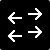
\includegraphics[width=.05\textwidth]{bisdn/switch}
        & switch     & \\ \hline 
            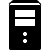
\includegraphics[width=.05\textwidth]{bisdn/host}
        & host     & \\ \hline 
        
\includegraphics[width=.05\textwidth]{bisdn/bond}
        & port     & \\
   \end{tabular}
\end{table}


%%----------------------------------------
%% Final materials
%%----------------------------------------

%% Bibliography
%% Comment the next command if BibTeX file not used
%% bibliography is in ``myrefs.bib''

\PrintBib{Thesus}

%% Index
%% Uncomment next command if index is required
%% don't forget to run ``makeindex thesis'' command
%\PrintIndex

\end{document}
